\section{Arduino IDE}
	Afin de développer le programme principal de la carte Arduino, nous avons utilisé le logiciel officiel Arduino IDE.
	\begin{figure}[H]
		\centering
		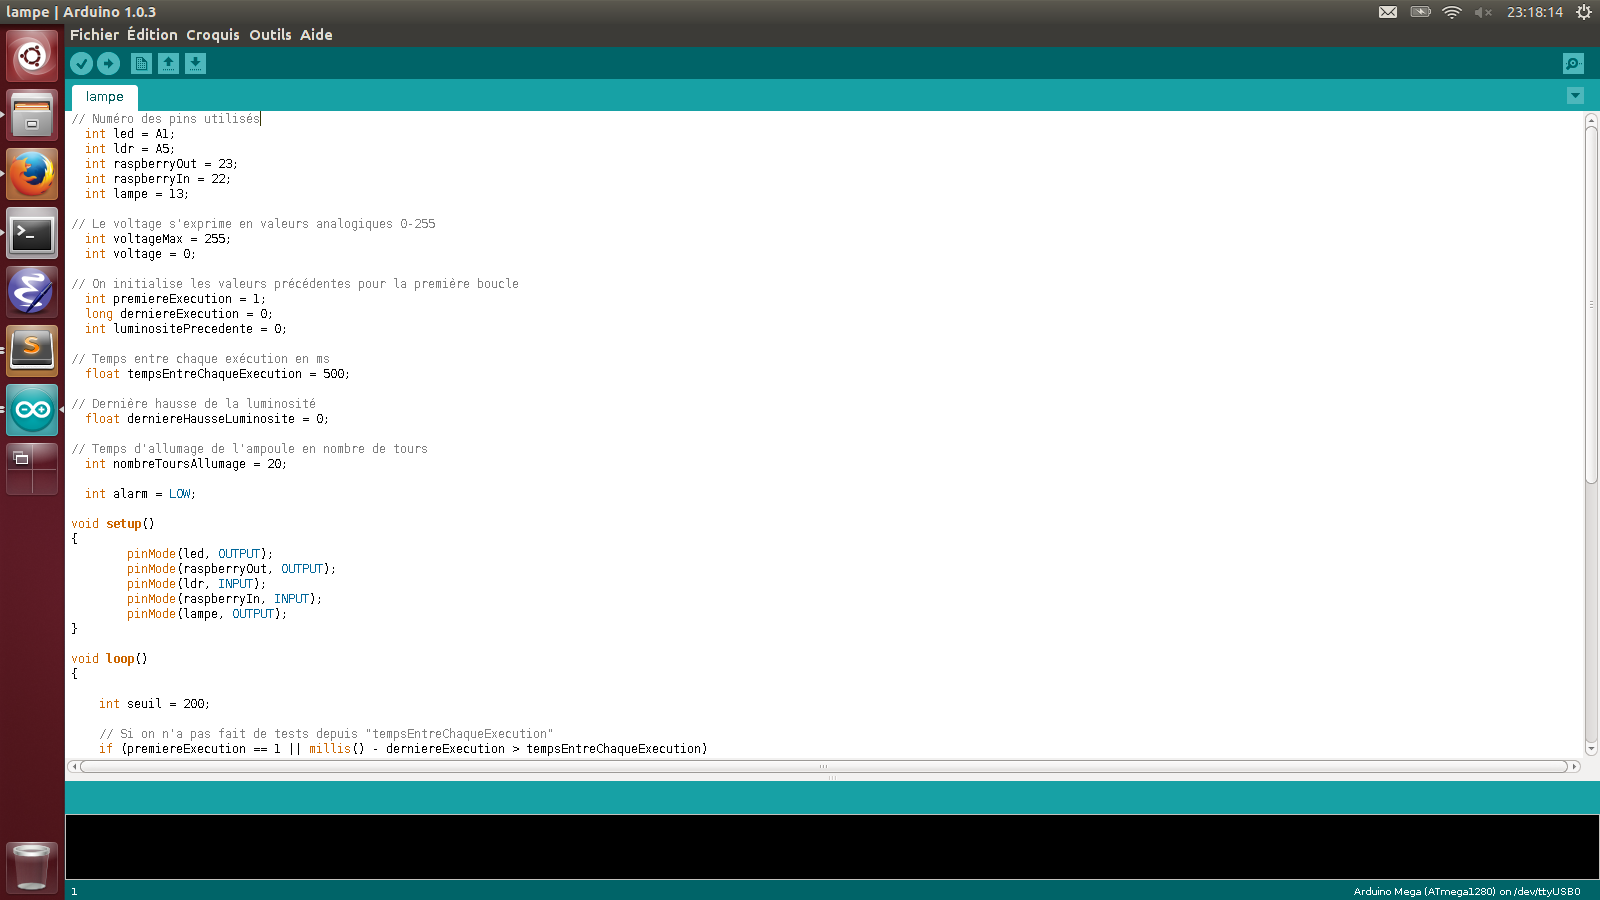
\includegraphics[width=350px]{images/arduinoIDE.png}
		\caption{Logiciel utilisé : Arduino IDE}
	\end{figure}

	La prise en main de ce logiciel c'est fait très simplement, c'est un éditeur de code simple. La seule subtilité rencontré à été de règler le modèle de la carte Arduino avant de transférer le programme sur la carte.

\section{Le langage Arduino}
	Le langage utilisé pour programmer la carte Aduino est un dérivé du langage C. Cette particularité nous a facilité la programmation des fonctionnalités de notre réveil intelligent grâce aux cours d'algorithmique donnés en parallèle en ASI3.

	Les limitations de langage ne nous ont posés aucun soucis. Les seules nouveautés à apréhender ont été les diverses connexions, lectures et écritures sur les pins de la carte Arduino.

\section{Le programme}
	Le programme installé sur la carte Arduino n'est pas très complexe mais nous avons tout fait pour le garder évolutif.\\

	Tout d'abord, le programme vérifie le pin d'entré provenant du Raspberry afin de savoir si l'alarme a été déclenché ou pas. Si c'est le cas, il va commencer l'allumage progressif de la LED en augmentant la valeur de sortie du pin de la LED. Dans un deuxième temps, la Arduino va vérifier la valeur envoyée par la photorésistance, si cette valeur dépasse un certain seuil (définit à 200 dans notre cas), le programme éteint la LED et envoie un signal sur le pin allant au Raspberry qui se chargera alors d'éteindre l'alarme.\\

	Ces instructions se répètent dans une boucle infinie. Afin d'éviter les pauses et que la carte Arduino soit toujours active, nous avons voulu ne pas utiliser la fonction "sleep". La carte Arduino fait donc tourner à son rythme la boucle, et les instructions sont déclenchées en fonction du temps écoulé. La variable tempsEntreChaqueExecution nous permet de réguler la vitesse de réponse de la carte Arduino. Cette astuce permet de rajouter très facilement des instructions pour un autre projet en rajoutant simplement une autre condition et une autre variable définissant un temps entre chaque exécution.\\

	Toujours dans un souci de garder le programme évolutif, nous n'avons pas inscrit en dur les informations concernant l'augmentation de voltage de la LED. Cette information est calculée à partir de deux variables, la première que nous venons d'évoquer est le \textit{tempsEntreChaqueExecution} et la deuxième est le \textit{nombreToursAllumage}. Grâce à ces deux variables nous pouvons calculer avec précision le temps d'allumage de la LED. Nous pouvons aussi règler la continuité de l'allumage (en diminuant le \textit{tempsEntreChaqueExecution} et en augmentant le \textit{nombreToursAllumage}) afin d'éviter de trop grand saut de voltage. Nous pouvons imaginer dans un nouveau projet une interface permettant à l'utilisateur de facilement règler les paramètres d'allumage de sa LED.\\

	Notre programme permet aussi de renseigner le voltage maximal si, par exemple, l'utilisateur ne veut pas que la LED s'allume complètement.
